\documentclass{article}
\usepackage[dutch]{babel}
\usepackage{graphicx}

\title{\Large Verslag \\ Proximity graphs}
\author{Mathijs Vos, Ramon Janssen, Petra van den Bos}

\begin{document}
\maketitle
\tableofcontents
\newpage

\begin{abstract}
Abstract hier
\end{abstract}

\section{Inleiding}
\emph{a short introduction about classification  in general and kNN and their applications.}\\

\section{Het Probleem}
\emph{say what is condensing and editing }\\
\subsection{Condensing en editing}

Het kNN-principe kan op een simpele manier op alle soorten gegevens worden toegepast. Door een nieuw punt simpelweg met alle punten in de trainingset te vergelijken kan een goed resultaat worden verkregen. In de praktijk levert dit echter problemen op in performance, omdat een dataset al snel veel dimensies en punten bevat. Ook wordt ruis daarmee overgenomen, omdat van elk punt van de trainingset wordt aangenomen dat deze correct gelabeld is. De complexiteit voor het testen van nieuwe punten wordt dan al snel veel te groot en daarvoor zijn optimalisaties vereist.\\

Het doel van condensing is om de grootte van een dataset te reduceren door redundante informatie te schrappen. Dit richt zich voornamelijk op gebieden waar zich veel punten met dezelfde klasse bevinden: de punten in het midden van het gebied voegen niets toe ten opzichte van de punten op de rand. Alleen de randen worden dus bespaard. Hierbij zorgt ruis voor een probleem, omdat één (verkeerd gelabeld) punt in het midden van een gebied er anders voor zou zorgen dat het midden niet meer condensed kan worden.\\
	
Voor het weghalen van ruis is er editing. Dit haalt punten weg die nabij veel punten met een andere classificatie liggen, omdat dit soort punten meer kans hebben om ruis te zijn. Dit kan het beste vóór het condensen gebeuren, zodat de condensing minder last heeft van ruis.\\
	
Voor zowel condensing als editing kan de precieze werking verschillen. Het is afhankelijk van het algoritme hoeveel informatie er verwijderd wordt. Als er meer informatie verwijderd wordt worden de resultaten gemiddeld slechter maar wordt de benodigde tijd voor het testen minder. Het verschilt ook per algoritme hoe effectief editing en condensing is onder verschillende omstandigheden, zoals de hoeveelheid dimensies en de vorm van de data.\\

\emph{The selected method: describe the method you selected: why this method, pseudo-code and characteristics you consider important}\\

\subsection{De methode}
De titel van het artikel dat wij gekozen hebben is: “Prototype selection for the nearest neighbour rulethrough proximity graphs”. We hebben dit artikel gekozen omdat het ons wel leuk leek om grafen te gebruiken en omdat het artikel duidelijk was. Er worden twee soorten grafen beschreven: ‘Gabriel Graphs’ en ‘Relative Neighbourhood Graph’. Beiden zijn grafen waarin punten verbonden worden door lijnen die elkaar niet snijden. Als een punt A verbonden is met punt B, is A een buur van B en B een buur van A.\\

In een Gabriel Graph is er een verbinding tussen twee punten, als binnen de cirkel, waarvan de verbinding de diameter is, geen andere punten liggen. Met de euclidische afstand kan dit formeel uitgedrukt worden: A en B hebben een verbinding als voor alle andere punten X: afstand2(A,B)<= afstand2(A,X) + afstand2(B,X). In figuur 1 zijn A en B verbonden, maar B en C niet. In figuur 2 is een gehele Gabriel Graph te zien. \\

\begin{center} 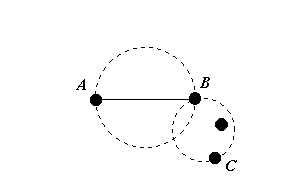
\includegraphics[keepaspectratio=true]{GGburen} \emph{Figuur 1} \end{center}

TODO: \\
Plaatje van gehele Gabriel Graph uit GraphVisualiser\\
Figuur  2\\

In een Relative Neighbourhood Graph hebben twee punten een verbinding als er geen andere punten binnen de ‘lune’ van die twee punten liggen, zie figuur 3. Met de euclidische afstand kan dit formeel uitgedrukt worden: A en B hebben een verbinding als voor alle andere punten X:  afstand(A,B) <= max\{afstand(A,X),afstand(B,X)\}. In figuur 3 zijn B en C  verbonden, maar A en B niet. In figuur 4 is een gehele Relative Neighbourhood Graph te zien.\\

\begin{center} 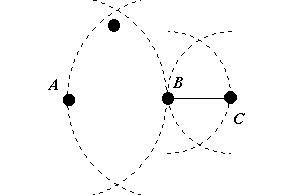
\includegraphics[keepaspectratio=true]{RNGburen} \emph{Figuur 3} \end{center}

TODO: \\
Plaatje van gehele Relative Neighbourhood Graph uit GraphVisualiser\\
Figuur 4\\

Deze grafen kun je gebruiken om nieuwe data (de testset) te classificeren aan de hand van data waarvan de classificatie al bekend is (de trainset). Een graaf bevat in eerste instantie dus alle punten uit de trainset. Om de performance te verbeteren en eventuele ruis te compenseren, wordt condensing en editing toegepast. Hierbij wordt gekeken naar de punten die een verbinding hebben met een bepaald punt. Bij condensing wordt ieder punt weggehaald, dat alleen verbindingen naar punten met dezelfde klasse heeft. In het artikel werden twee soorten editing algoritmes besproken: een eerste orde editing algoritme en een tweede orde editing algoritme. Het eerste orde editing algoritme bepaald voor elk punt of de meerderheid van de buren van dat punt van een bepaalde, andere klasse is. De punten waarvoor dit geldt, worden verwijderd. Het tweede orde algoritme verwijderd alle punten waarvoor geldt dat de meerderheid van de buren van een bepaalde, andere klasse is, en als ook de meerderheid van de buren van die buren van een bepaalde, andere klasse is.

\section{Experimenten}
\emph{Report results of experiments with the selected method on the considered datasets, 
in particular accuracy and storage reduction reduction. }\\
\emph{Discuss the performance of the selected method.}\\

\section{Conclusie}
\emph{Summarize the content of your report and provide some conclusive remarks and observation about the effectiveness of the selected method and possible future work (improvements).} \\
\end{document}